\section{Example Scenario}
\label{sec:Example}

\begin{figure*}
    \centering
    \begin{subfigure}[b]{0.45\textwidth}
			\centering
      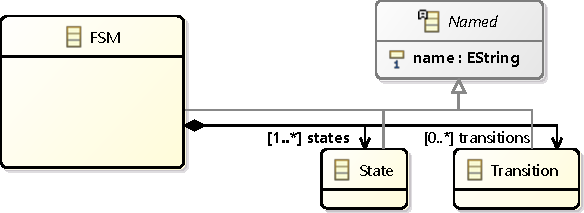
\includegraphics[width=\textwidth]{FSM0.pdf}
      \caption{Initial \metamodel.}
      \label{fig:FSM:Init}
    \end{subfigure}
    \hfill
    \begin{subfigure}[b]{0.45\textwidth}
			\centering
      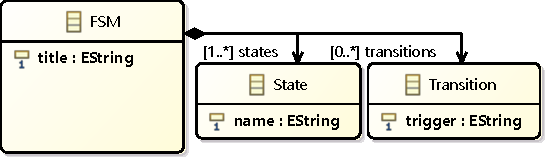
\includegraphics[width=\textwidth]{FSM1.pdf}
      \caption{\textbf{Step 1:} Specifying relevant \textsf{name}s}
      \label{fig:FSM:Relevant}
    \end{subfigure}
    \hfill
    \begin{subfigure}[b]{0.45\textwidth}
			\centering
      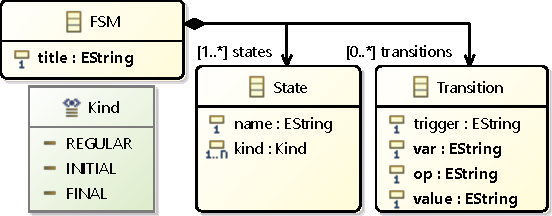
\includegraphics[width=\textwidth]{FSM2.pdf}
      \caption{\textbf{Step 2:} Adding rudimentary guards and \textsf{FINAL}. \LK{\textsf{FINAL} is not yet included in the image.}}
      \label{fig:FSM:Guard}
    \end{subfigure}
    \hfill 
		\begin{subfigure}[b]{0.45\textwidth}
			\centering
      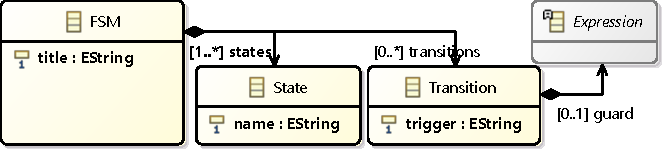
\includegraphics[width=\textwidth]{FSM3.pdf}
      \caption{\textbf{Step 3:} Specifying a fully-fledged \textsf{Expression} for \textsf{guard}s.}
      \label{fig:FSM:Expression}
    \end{subfigure}
    \caption{Three evolution steps for the \textsf{FSM} \metamodel. Note that details, such as the state kind, are omitted in subfigure b.}%\LC{Well, they aren't part of that MM yet, right? State kind only gets introduced in Step 2 so Subfigure c, right?}\LK{But they are already in subfigure a and the text mentions that some details are omitted in subfigure b.}}
    \label{fig:FSM}
\end{figure*}

This Section describes a small, yet representative example of \metamodel
evolution steps on a popular \textsc{Dsl}, the Finite State Machine (\textsf{FSM}).
Note that we simplify the \metamodels and corresponding \viewtypes, to focus 
the discussion only on the parts relevant to co-evolution. 

A methodologist starts with the simple version depicted in \cref{fig:FSM:Init}:
an \textsf{FSM} consists of \textsf{State}s and \textsf{Transition}s. Each class
inherits a \textsf{name} that denotes the \textsf{FSM}'s title, the \textsf{State}'s
name, and the \textsf{Transition}'s trigger. Moreover, \textsf{INITIAL} \textsf{State}s
are distinguished from \textsf{REGULAR} ones to indicate where computations start.
From this initial version, the methodologist defines a \viewtype \textsf{VT\_FSM}
that has two characteristics (cf. \cref{fig:VT}). First, it captures \textsf{Transition}s \emph{inside},
or as part of, \textsf{State}s, to help compute e.g. the set of outgoing 
\textsf{Transition}s from a given \textsf{State}. Second, it represents the various
\textsf{kind}s of \textsf{State}s as a hierarchy, instead of an enumeration,
in order to facilitate the specification of a future visual concrete syntax where
each class is associated to a specific icon.
Additionally, \textsf{VT\_FSM} explicitly computes \textsf{nbStates} and 
\textsf{nbTransitions}, the number of \textsf{State}s and \textsf{Transition}s 
in any given \textsf{FSM} conformant model. A \emph{textual} concrete syntax 
provides a view, conformant to \textsf{VT\_FSM}, of a \textsf{Simple FSM} containing
four \textsf{State}s and six \textsf{Transition}s.


In a first evolution step, the methodologist refines the \textsf{FSM} metamodel,
after noticing that the inherited \textsf{name}s actually play different roles,
by  \emph{pushing down} the \textsf{name} attribute and \emph{renaming} it where
appropriate (other irrelevant details are omitted from \cref{fig:FSM:Relevant}). 
This evolution step does not impact the \viewtypes, but rather the way information
in views is computed: for example, the \textsf{name} of a \textsf{Transition} in
\textsf{VT\_FSM} can no longer be computer using \texttt{t.name} (where 
$\mathsf{t : FSM::Transition}$), but rather with \texttt{t.\textbf{trigger}}. 
The methodologist can take this further by reflecting the \textsf{name}s update
into \textsf{VT\_FSM} to avoid further confusion and keep a direct link with
\textsf{FSM}'s meta-elements.

In a second evolution step, the methodologist wants to extend \textsf{FSM}'s 
behaviour in two ways, leading to the version depicted in \cref{fig:FSM:Guard}. First, by adding \textsf{FINAL} \textsf{State}s,
resulting in \emph{creating} the enumeration literal \textsf{FINAL}.
Second, by adding a rudimentary representation for guards that may prevent 
triggering a \textsf{Transition} when its guard evaluates to \texttt{false}. 
For this purpose, three new attributes are \emph{created} in \textsf{Transition}, allowing to capture
simple expressions over \textsf{var}iables, using boolean and numeric \textsf{value}s
(e.g., \textsf{v = 10} or \textsf{k or l}). After this step, \textsf{VT\_FSM}'s
models may still be valid w.r.t.~the evolved \metamodel (assuming the lack of 
guard is interpreted as a trivial \textsf{true} guard),
but \viewtypes likely have to reflect this new information by \emph{ADD}ing new entities in appropriate places.

In a final evolution step, the methodologist, confident with the implemented
execution engine, specifies a fully-fledged \textsf{Expression} model,
allowing a \textsf{Transition} to possess a \textsf{guard}, thus \emph{deleting}
the extra attributes added in the previous step. \cref{fig:FSM:Expression} depicts the resulting \metamodel.
\LK{How does this relate to the view type?}

% \HM{I think it might be useful to mention the operators from Table \cref{tab:suggestions} applied to the MM at each step and later connect this with the suggestions?}

\begin{figure}
    \centering
    \begin{subfigure}[b]{\columnwidth}
			\centering
      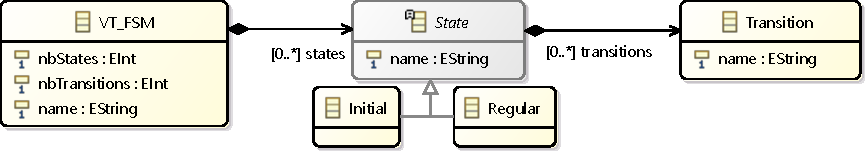
\includegraphics[width=\columnwidth]{FSM_VT.pdf}
      \caption{A \viewtype for \textsf{FSM}, with \textsf{Transition} \emph{inside} \textsf{State}s.\LC{Similar comment to LK's on Figure 2 caption: Final subclass of State should be added?}}
      \label{fig:VT:VMM}
    \end{subfigure}
    \hfill
    \begin{subfigure}[b]{\columnwidth}
			\centering
      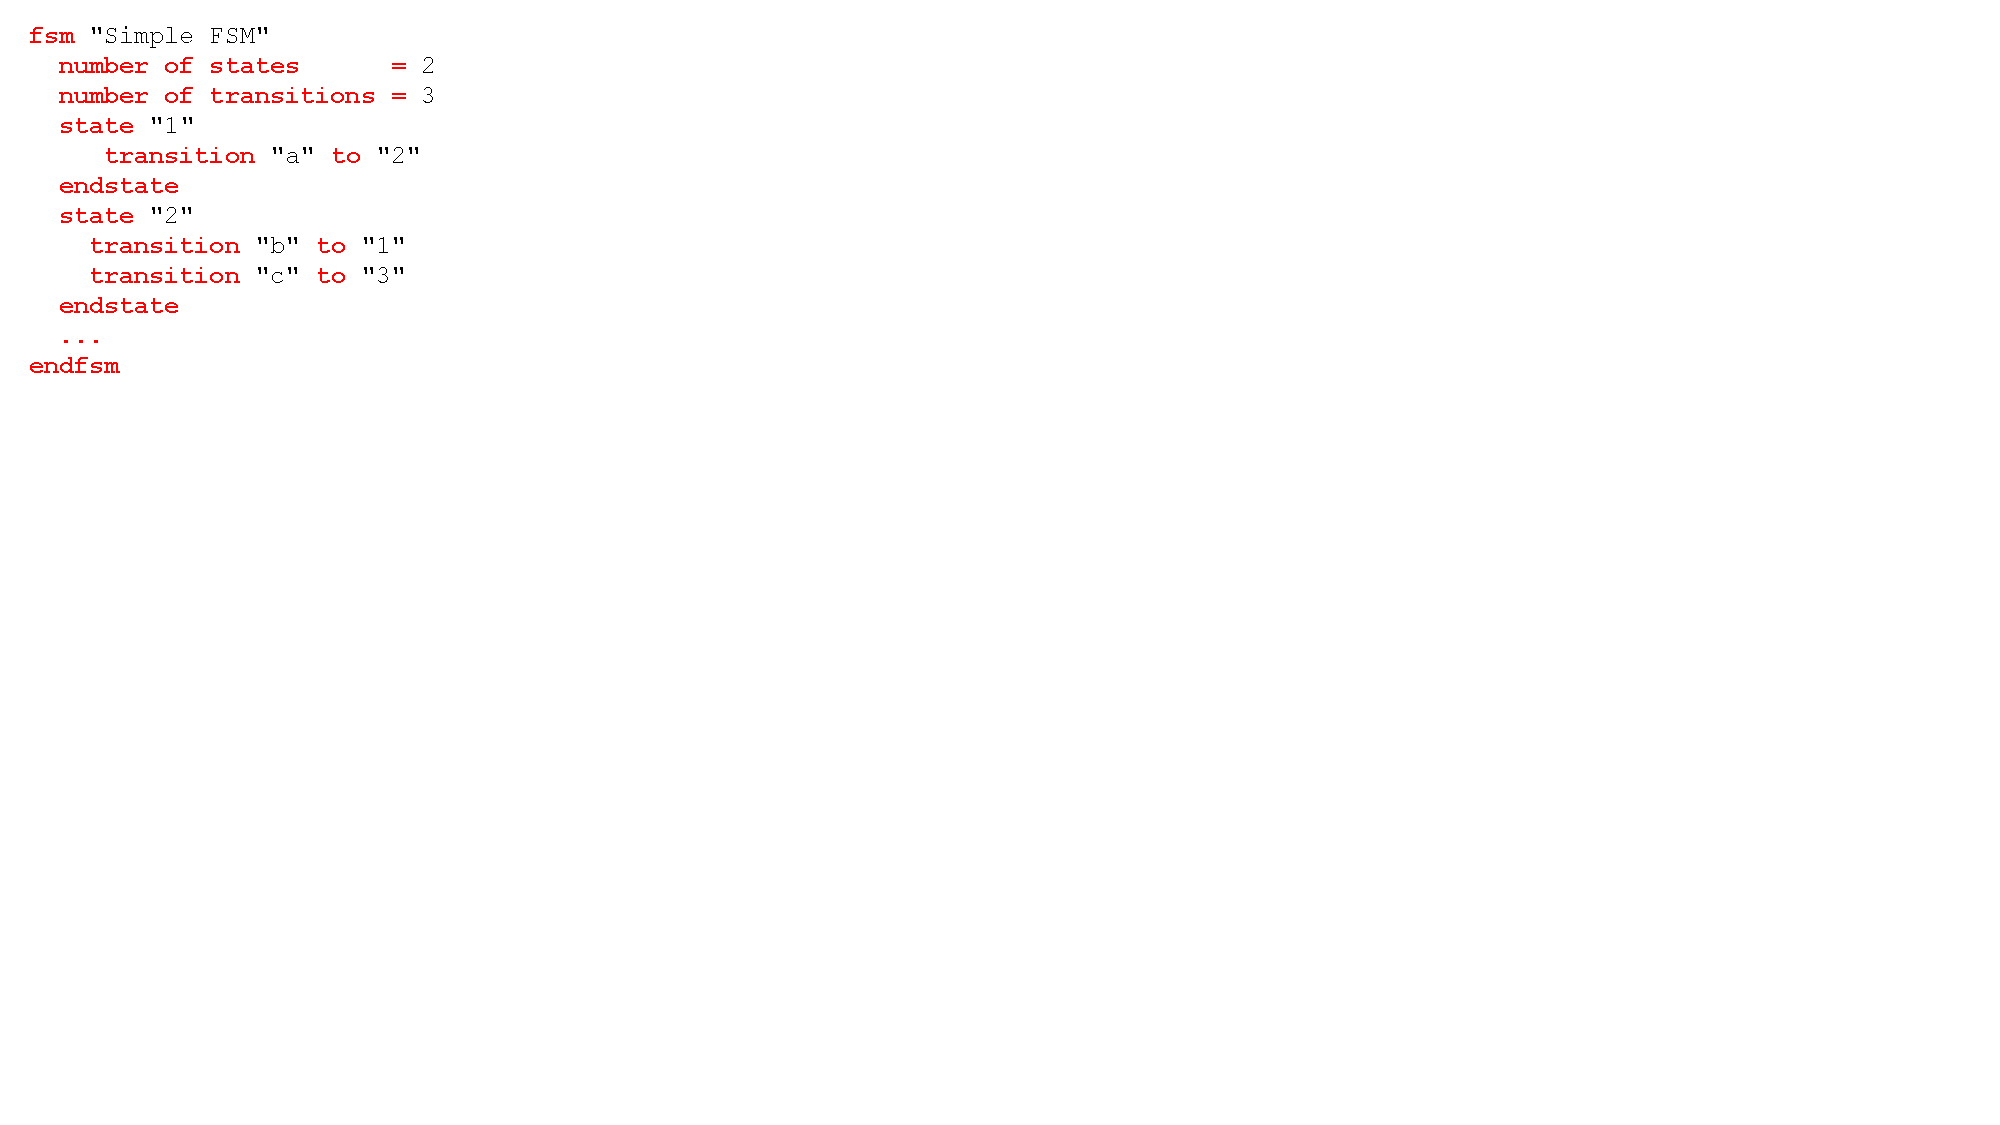
\includegraphics[width=0.5\textwidth, page=1, clip, trim=0cm 12cm 26cm 0cm]{VT.pdf}
      \caption{A textual view of an \textsf{FSM} model named \textsf{Simple FSM} with 4 \textsf{States} and 6 \textsf{Transitions} (details omitted).}
      \label{fig:VT:TM}
    \end{subfigure}
    \caption{A \Viewtype, and an associated view for the \textsf{Simple FSM} model.}
    \label{fig:VT}
\end{figure}
